\documentclass{beamer}

\usepackage[utf8]{inputenc}
\usepackage{default}
\usepackage{pifont}
\usepackage{multimedia}

\usepackage{listings}
\lstset{language=C++}

\usepackage{verbatim}

% for the \hat command (unit vectors)
\usepackage{amsmath}

\usepackage{pgfplots}
\usepackage{tikz}
\usetikzlibrary{calc}
\usetikzlibrary{positioning}

\usepgflibrary{fpu}
\usepgfplotslibrary{external} 

\tikzexternalize
\pgfplotsset{compat=1.8}

\usepackage{subcaption}
\captionsetup{compatibility=false}

\usepackage{comment}

\usepackage{multimedia}
\usetikzlibrary{fit}

\usetheme{Boadilla}
%\usecolortheme{orchid}
\usecolortheme{orchid}

\definecolor{tecnico}{RGB}{0, 145, 218}
\setbeamercolor{structure}{fg=tecnico}

\title[Autonomous Systems Course]{Autonomous Systems \& Introduction to Robotics}
\subtitle{ROS practical session}
\author[Rute Luz]{Rute Luz \\ {\tiny (Oscar Lima \& Carlos Azevedo)}}
\institute[ISR]{ISR: Institute for Systems and Robotics\\LARSyS: Laboratory for Robotics and Engineering Systems\\IST: Instituto Superior T\'ecnico, Lisboa Portugal}


\titlegraphic{\centering\includegraphics[height=1.7cm]{logos/isr-lisboa-logo.png}\hspace*{0.0cm}\includegraphics[height=1.8cm]{logos/larsys_logo_new.png}\hspace*{0.0cm}\includegraphics[height=1.5cm]{logos/ist-logo.png}}

\begin{document}

%---------------------------------------------

\begin{frame}
\titlepage
\end{frame}

%---------------------------------------------

\begin{frame}{tf\footnote{\url{http://wiki.ros.org/tf}}}
		
	\begin{itemize}
		\item Material from this slides was borrowed from here\footnote{\url{https://www.ethz.ch/content/dam/ethz/special-interest/mavt/robotics-n-intelligent-systems/rsl-dam/ROS2017/lecture3.pdf}}
		\item tf is a tool for keeping track of coordinate frames over time.
		\item Lets the user transform points, vectors, etc. between coordinate frames at desired time.
		\item Implemented as publisher-subscriber model on the topics /tf and /tf\_static
		\item New tf2 api can be consulted here\footnote{\url{http://wiki.ros.org/tf2}}
	\end{itemize}

\end{frame}

%---------------------------------------------

\begin{frame}{tf simple example (1)}
	
	% one image
	\begin{figure}[H]
		\centering
		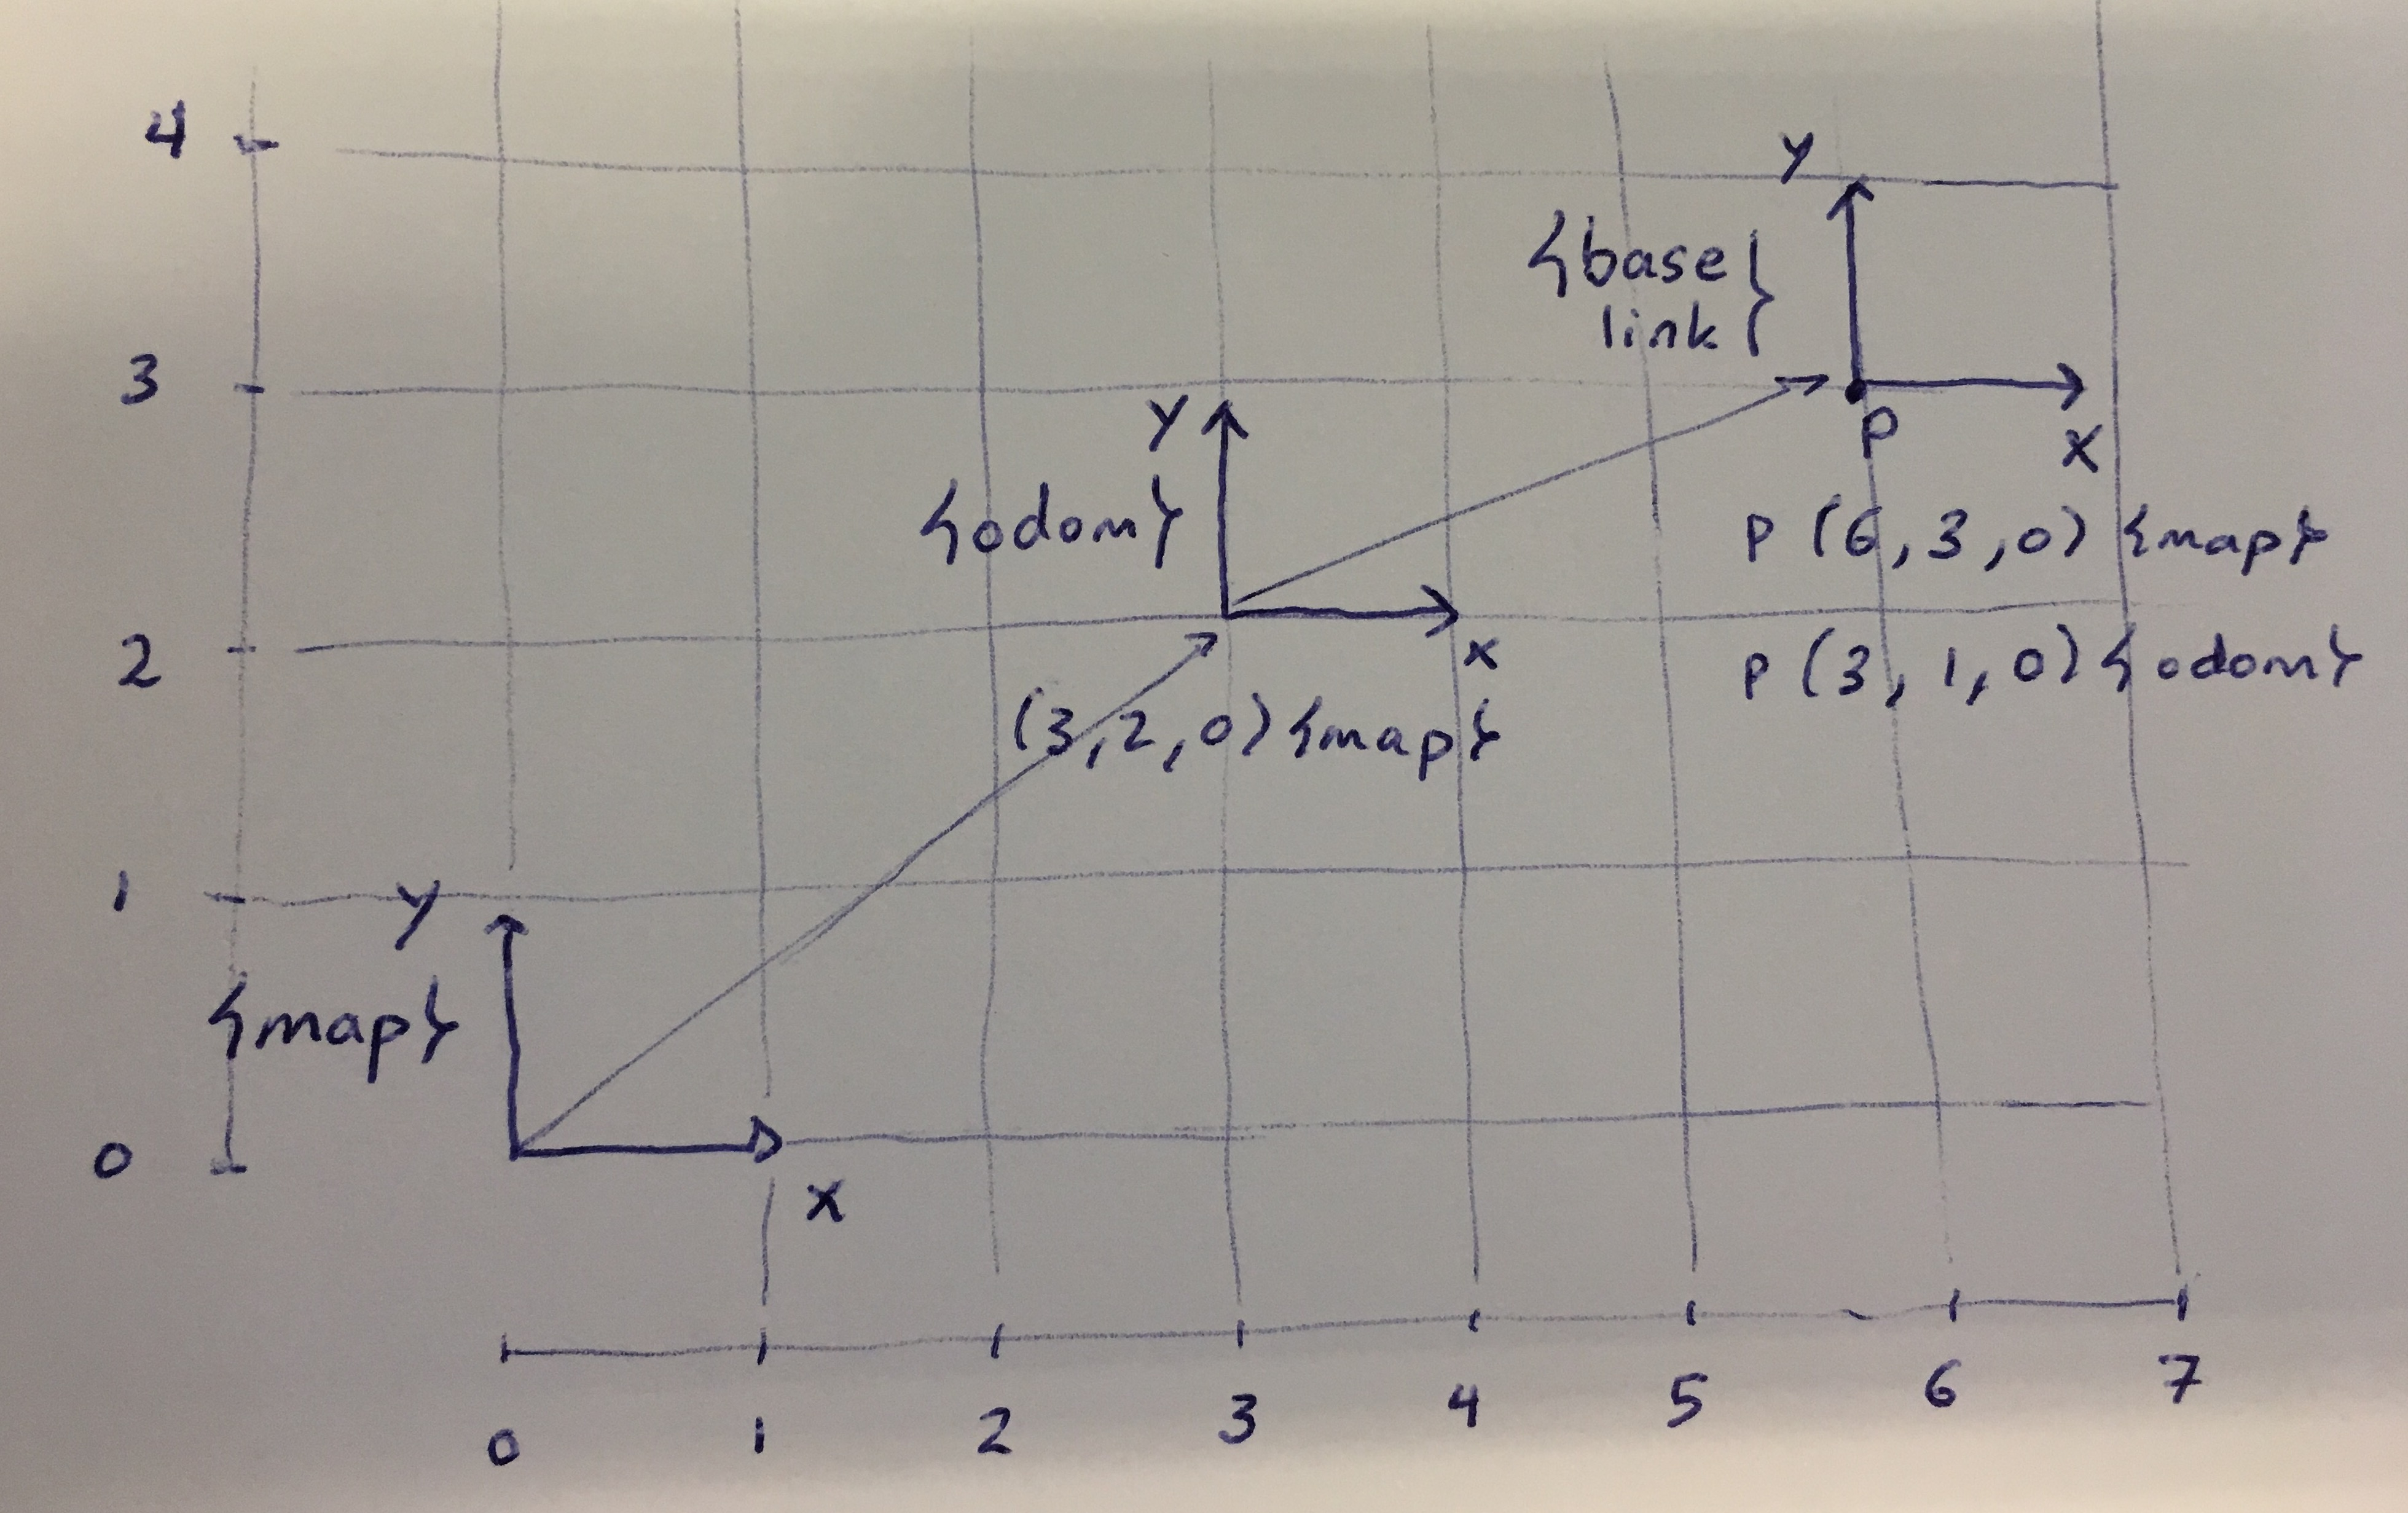
\includegraphics[height=6.0cm]{images/tf_simple_example.jpg}
	\end{figure}
	
\end{frame}

%---------------------------------------------

\begin{frame}{tf simple example (2)}
	
	\begin{itemize}
		\item On rviz it looks like this
	\end{itemize}
	
	% one image
	\begin{figure}[H]
		\centering
		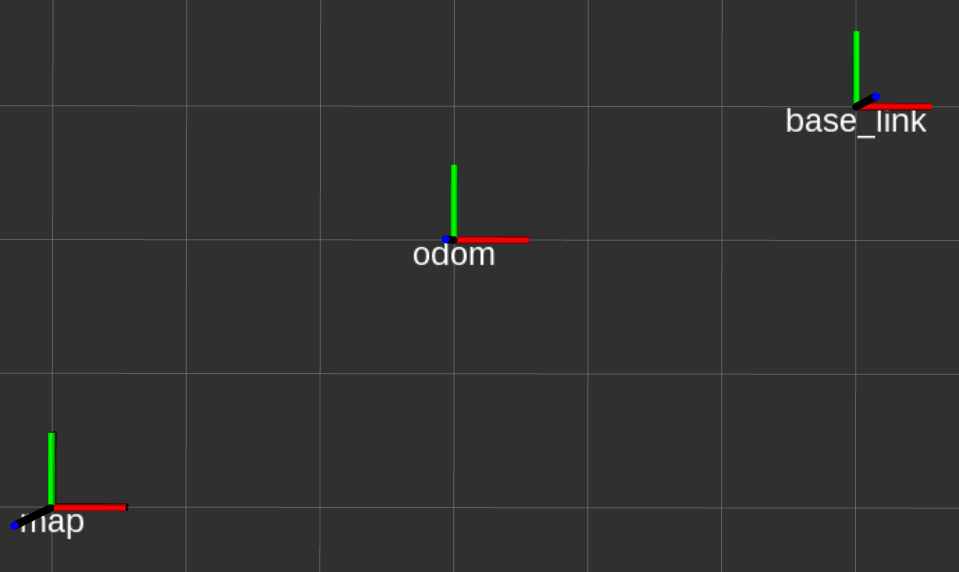
\includegraphics[height=5.0cm]{images/rviz_visualization.png}
	\end{figure}
	
\end{frame}

%---------------------------------------------

\begin{frame}{tf}
	\begin{itemize}
		\item A real world example (mbot robot)
	\end{itemize}
	
    % one image
	\begin{figure}[H]
		\centering
		\includegraphics[height=6.0cm]{images/mbot_frames.png}
	\end{figure}
	
\end{frame}

%---------------------------------------------

\begin{frame}{tf \footnote{\url{http://wiki.ros.org/tf}}}
	\begin{itemize}
		\item Example tf tree for simulated pioneer + wall-e robot
	\end{itemize}
	
	%	% one image
	\begin{figure}[H]
		\centering
		\includegraphics[height=6.0cm]{images/tf_tree_example.png}
	\end{figure}
	
\end{frame}

%---------------------------------------------

\begin{frame}{Pioneer P3-DX robot\footnote{\url{http://www.mobilerobots.com/ResearchRobots/PioneerP3DX.aspx}}}
	\begin{itemize}
		\item Differential drive robot
		\item Weight: 9kg, max. speed: 1.2 m/s
		\item battery time: 8 hours w/ 3 batteries
		\item Front sonar ring
		\item All robots in the lab are equipped with a USB to serial converter
	\end{itemize}
	
	% one image
	\begin{figure}[H]
		\centering
		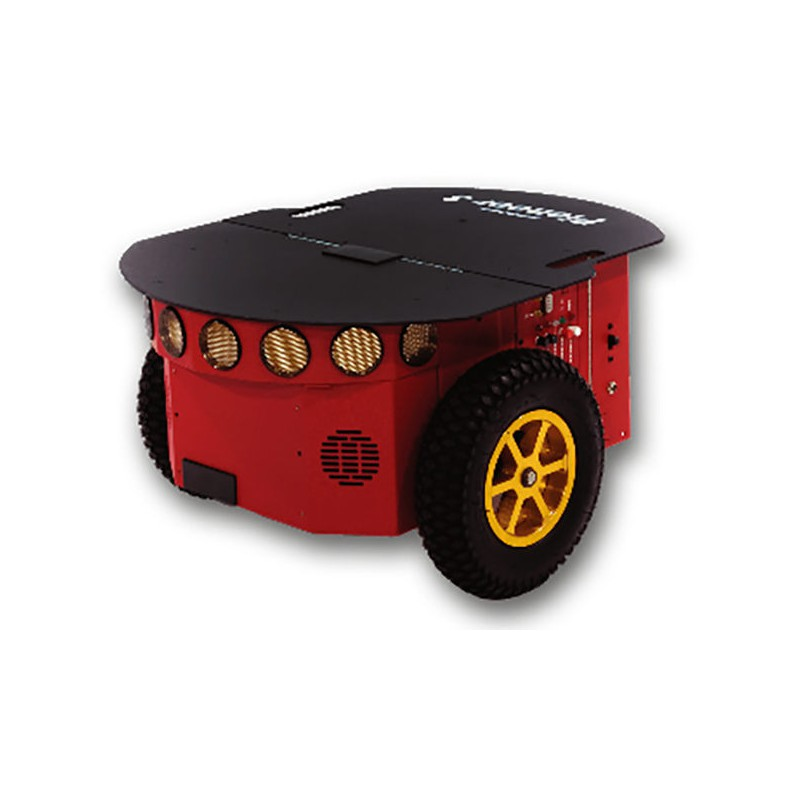
\includegraphics[height=5.0cm]{images/pioneer_P3-DX_robot.jpg}
	\end{figure}
	
\end{frame}

%---------------------------------------------

%\begin{frame}{AMCL}
%	\begin{itemize}
%		\item Follow README
%	\end{itemize}
%	
%	% one image
%%	\begin{figure}[H]
%%		\centering
%%		\includegraphics[height=9cm]{images/corner_problem.pdf}
%%	\end{figure}
%	
%\end{frame}

%---------------------------------------------

%\begin{frame}{GMapping}
%	\begin{itemize}
%		\item todo
%	\end{itemize}
%	
%	% one image
%	%	\begin{figure}[H]
%	%		\centering
%	%		\includegraphics[height=9cm]{images/corner_problem.pdf}
%	%	\end{figure}
%	
%\end{frame}

%----------------------------------------------

%\begin{frame}{rosbag}
%	\begin{itemize}
%		\item use\_sim\_time parameter, and —clock option for rosbag
%	\end{itemize}
%	
%	% one image
%	%	\begin{figure}[H]
%	%		\centering
%	%		\includegraphics[height=9cm]{images/corner_problem.pdf}
%	%	\end{figure}
%	
%\end{frame}

%---------------------------------------------

\begin{frame}
\begin{LARGE}
\begin{center}
Thank you!\\

Questions? :)\\

\vspace*{1cm}

\footnotesize
If you have a question please create a Github issue so that we can all benefit from the posted answers under:
\\
\url{https://github.com/socrob/autonomous\_systems/issues}

\vspace*{2cm}
\end{center}
\end{LARGE}
\end{frame}

%---------------------------------------------

\end{document}